\documentclass[14pt]{beamer}
\usetheme{Dresden}
\usecolortheme{orchid}

\usepackage{xcolor}
\usepackage{listings}
\usepackage{courier}
\usepackage{graphicx}
\usepackage{amsmath}
\usepackage{algorithm2e}
\usepackage{multicol}

\usefonttheme[onlymath]{serif}

\definecolor{mGreen}{rgb}{0,0.6,0}
\definecolor{mGray}{rgb}{0.5,0.5,0.5}
\definecolor{mPurple}{rgb}{0.8,0,0.82}
\definecolor{backgroundColour}{rgb}{0.95,0.95,0.92}
\definecolor{lightBlue}{rgb}{0.1, 0.1, 0.8}

\lstdefinestyle{CStyle}{
    backgroundcolor=\color{backgroundColour},   
    commentstyle=\color{mGreen},
    keywordstyle=\color{magenta},
    numberstyle=\tiny\color{mGray},
    stringstyle=\color{mPurple},
    basicstyle=\footnotesize\ttfamily,
    breakatwhitespace=false,         
    breaklines=true,                 
    captionpos=b,                    
    keepspaces=true,                 
    numbers=left,                    
    numbersep=5pt,                  
    showspaces=false,                
    showstringspaces=false,
    showtabs=false,                  
    tabsize=2,
    language=C
}

\lstdefinestyle{Ctable}{
    backgroundcolor=\color{backgroundColour},   
    commentstyle=\color{mGreen},
    keywordstyle=\color{magenta},
    numberstyle=\tiny\color{mGray},
    stringstyle=\color{mPurple},
    basicstyle=\footnotesize\ttfamily,
    breakatwhitespace=false,         
    breaklines=true,                 
    captionpos=b,                    
    keepspaces=true,                                  
    showspaces=false,                
    showstringspaces=false,
    showtabs=false,                  
    tabsize=2,
    language=C
}

\lstdefinestyle{pseudo}{
        basicstyle=\ttfamily\footnotesize,
        keywordstyle=\color{lightBlue},
        morekeywords={BEGIN,END,IF,ELSE,ENDIF,ELSEIF,PRINT,WHILE,RETURN,ENDWHILE,DO,FOR,TO,IN,ENDFOR,BREAK,INPUT,READ},
        morecomment=[l]{//},
        commentstyle=\color{mGreen}
}

\lstset{basicstyle=\footnotesize\ttfamily,breaklines=true}
\lstset{framextopmargin=50pt,tabsize=2}

\title{ENGG1003 - Friday Week 2}
\subtitle{Fixing the Mistakes I Made on Tuesday\\Lets do Some Examples}
\author{Brenton Schulz}
\institute{University of Newcastle}
\date{\today}

\begin{document}
\titlepage

\begin{frame}
\frametitle{Example: Testing Factors}
Task: Write a C program which reads two integers from the user and tests if the second is a factor of the first, printing the result.\\
\vspace{5mm}
Eg: If the user enters 12 and 3 the program would print something like:\\
\texttt{3 is a factor of 12}
\end{frame}

\begin{frame}[fragile]
\frametitle{Example: Testing Factors}
Lets convert the problem down into ``high level'' pseudocode:
\begin{lstlisting}[style=pseudo]
BEGIN
	integer x
	integer y
	READ x from the user
	READ y from the user
	Test if y is a factor of x
	Tell the user the result
END
\end{lstlisting}
Can every line of pseudocode be turned into C? How are we going to test if one number is a factor of another?
\end{frame}

\begin{frame}
\frametitle{Example: Testing Factors}
Lets make an attempt at factor testing, perhaps start with:\\
\vspace{5mm}
Definition: \textit{Factors} are numbers we can multiply together to make another number. Eg: 2 and 3 are factors of 6 as $2 \times 3 = 6$.\\
\vspace{5mm}
Is this definition useful for this problem? Is it easy to turn this definition into C code?
\end{frame}

\begin{frame}
\frametitle{Example: Testing Factors}
No, not really. C can't easily do ``can I find another integer that multiplies with $y$ to make $x$''. That instruction is not \textit{executable}. \\
\vspace{5mm}
Lets try again: \\
\vspace{5mm}
An integer, $y$, is a factor of a number, $x$, if the integer evaluation of $x\div y$ has no remainder.\\
\vspace{5mm}
Can \textit{this} become C code?
\end{frame}

\begin{frame}[fragile]
\frametitle{Example: Testing Factors}
YES! We can use the modulus operator, \texttt{\%}, to test if a division has a remainder with the code:

\begin{lstlisting}[style=CStyle]
if( (x % y) == 0) {
	// y is a factor of x
}
\end{lstlisting}

\end{frame}

\begin{frame}[fragile]
\frametitle{Modulus Example - Factor Testing}
With this fact, lets tweak the pseudocode:
\begin{lstlisting}[style=pseudo]
BEGIN
	integer x
	integer y
	READ x from the user
	READ y from the user
	IF (x % y) == 0
		PRINT y is a factor of x
	ELSE
		PRINT y is NOT a factor of x
	ENDIF
END
\end{lstlisting}
\end{frame}

\begin{frame}[fragile]
\frametitle{Modulus Example - Factor Testing}
...and convert each line to C:\\
\vspace{4mm}
\small{(\texttt{printf();} output changed to fit on slide)}\\
\small{(C Code is almost missing \texttt{\#include <stdio.h>})}
\vspace{-2mm}
\begin{table}[H]
\centering

\begin{tabular}{ll}
Pseudocode & C Code \\
\hline

\begin{lstlisting}[style=pseudo,basicstyle=\ttfamily\scriptsize]
BEGIN
	integer x
	integer y
	READ x from the user
	READ y from the user
	IF (x % y) == 0
		PRINT y is a factor
	ELSE
		PRINT y isn't a factor
	ENDIF
END
\end{lstlisting} &

\begin{lstlisting}[style=Ctable,basicstyle=\ttfamily\scriptsize]
int main() {
	int x;
	int y;
	scanf("%d", &x);
	scanf("%d", &y);
	if( (x % y) == 0) {
		printf("%d is a factor\n", y);
	} else {
		printf("%d isn't factor\n", y);
	}
}
\end{lstlisting}
\\

\hline
\end{tabular}
\end{table}

\end{frame}


\begin{frame}[fragile]
\frametitle{Modulus Example - Code with Prompt}
\begin{lstlisting}[style=CStyle,caption=\texttt{factorTest.c}]
#include <stdio.h>
int main() {
	int x, y;
	printf("Enter an integer: ");
	scanf("%d", &x);
	printf("Enter another integer: ");
	scanf("%d", &y);
	if(x % y == 0) { // ie: if the remainder is zero
		printf("%d is a factor of %d\n", y, x);
	} else {
		printf("%d is NOT a factor of %d\n", y, x);
	}
	return 0;
}
\end{lstlisting}
\end{frame}

\begin{frame}
\frametitle{Factor Testing Discussion}
\begin{itemize}
\item Is this code \textit{robust}?
\item Can the user enter numbers which make the code produce the wrong number?
\item What happens if $\texttt{y}>\texttt{x}$?
	\begin{itemize}
		\item It might be fine, it might not. Have a think about it and do some testing in the lab
	\end{itemize}
\item Get in the habit of testing code, both with ``expected'' input and ``weird'' input
\item What happens if you enter letters instead of numbers? Or negatives? Or ask where the bathroom is?
\end{itemize}
\end{frame}

\begin{frame}
\frametitle{Modulus Example 2 - Factorisation}
\begin{itemize}
\item We now know how to test if a number is a factor of another
\item What about a full factorisation?
\end{itemize}

\textbf{Task:} Write a C program which reads an integer from the user and outputs all of its factors.
\end{frame}

\begin{frame}
\frametitle{Modulus Example 2 - Factorisation}
\begin{itemize}
\item How does factorisation happen, anyway?
	\begin{itemize}
		\item Normally? In your head. ``Dream up'' the answer.
		\item On a computer? We need to \textit{brute force} it.
			\begin{itemize}
				\item ie: Simply test every integer which might work	
			\end{itemize}
		\item All factors of a number, $k$ are in the range [1,k]
			\begin{itemize}
				\item 1 and k are always factors, so explicitly testing them is optional
			\end{itemize}
		\item They are also all integers
		\item Thankfully, this is a finite number of tests
	\end{itemize}
\item Faster algorithms \textit{might} exist
	\begin{itemize}
		\item You would need to consult number theory literature
		\item This is beyond my (Brenton's) knowledge
	\end{itemize}
\end{itemize}
\end{frame}

\begin{frame}
\frametitle{Modulus Example 2 - Factorisation}
\begin{itemize}
\item How can we test lots of numbers?
	\begin{itemize}
		\item The program needs to count
		\item The input is unknown, so we need a loop
		\item ie: we can't ``hard code'' counting when  we don't know when to stop!
	\end{itemize}
\end{itemize}
\end{frame}




\begin{frame}[fragile]
\frametitle{Modulus Example - Factorisation}
Lets write some pseudocode for the factorisation problem. We start with something really ``high level'':
\begin{lstlisting}[style=pseudo]
BEGIN
	Integer x
	READ a value for x from the user
	Calculate x's factors
	PRINT x's factors
END
\end{lstlisting}
\end{frame}


\begin{frame}[fragile]
\frametitle{Modulus Example - Factorisation}
Now lets \textit{imply} a loop, but not explicitly write it:
\begin{lstlisting}[style=pseudo]
BEGIN
 Integer x
 READ a value for x from the user
 Test if every integer from 1 to x is a factor of x
 PRINT x's factors
END
\end{lstlisting}
\end{frame}

\begin{frame}[fragile]
\frametitle{Modulus Example - Factorisation}
\begin{itemize}
	\item How do we code ``Test if every integer from 1 to x is a factor of x''?
	\item Well, we know how to test one integer, \texttt{n}:\\ \texttt{if( x \% n == 0)}
	\item How do we \textit{count?}
	\item With what we know so far? A \texttt{while()} loop!

\begin{lstlisting}[style=pseudo]
integer count = 1
WHILE count <= n
	count = count + 1 // Counts from 1 to n
ENDWHILE
\end{lstlisting}
	\item A ``better'' method will be shown later
\end{itemize}
\end{frame}

\begin{frame}[fragile]
\frametitle{Modulus Example - Factorisation}
\begin{lstlisting}[style=pseudo]
BEGIN
	integer x
	integer count = 1
	READ a value for x from the user
	WHILE (count <= x)
 		IF (x % count) == 0
 			PRINT <count> is a factor of <x>
		ENDIF
		count = count + 1
	ENDWHILE
END
\end{lstlisting}
\end{frame}

\begin{frame}
\frametitle{Modulus Example - Factorisation}
\begin{itemize}
\item Notice the \texttt{PRINT} statement \textit{inside} the loop
	\begin{itemize}
		\item Previous pseudocode has factorisation and printing as different steps
	\end{itemize}
\item This means we don't need to remember a list of factors as we go
\item We will learn how to work with lists later
	\begin{itemize}
		\item C calls a list of variables an \textit{array}
	\end{itemize}
\item Lets read and run the final program...
\end{itemize}
\end{frame}

\begin{frame}[fragile]
\frametitle{Modulus Example - Factorisation}
\begin{lstlisting}[style=CStyle,basicstyle=\ttfamily\footnotesize,caption=\texttt{factors.c}]
#include <stdio.h>
int main() {
	int count = 1, x;
	printf("Enter an integer to factorise: ");
	scanf("%d", &x);
	while(count <= x) {
		if(x % count == 0) // If the remainder is zero
			printf("%d is a factor of %d\n", count, x);
		count++;
	}
	return 0;
}
\end{lstlisting}
\end{frame}

\begin{frame}[fragile]
\frametitle{Modulus Example - Factorisation}
Example output:
\begin{lstlisting}[style=pseudo]
Enter an integer to factorise: 76545478
1 is a factor of 76545478
2 is a factor of 76545478
38272739 is a factor of 76545478
76545478 is a factor of 76545478
\end{lstlisting}

Is it correct? Check output with \underline{\href{https://www.wolframalpha.com/input/?i=factors+of+76545478}{Wolfram Alpha}}
\\
\vspace{5mm}
Observation: A modified version of this code (with \texttt{unsigned int}) only takes 15 seconds to factorise 4294967294
\end{frame}

\begin{frame}
\frametitle{Discussion}
\begin{itemize}
\item Pay close attention to the value of \texttt{count}
\item It is initialised to 1
\item It is used \textit{before} incrementing it
\item Incrementing is the last thing in the loop
\item The loop \textit{condition} is ``less than \textit{or equal to}'' so that \texttt{x} itself is explicitly tested as a factor
	\begin{itemize}
		\item Remember that 1 and x are always factors of x? 
	\end{itemize}
\end{itemize}
\end{frame}

\begin{frame}
\frametitle{Case Study: Calulating $\pi$}
Consider a quadrant of a unit circle ($r=1$) with a square around it:
\begin{columns}
\begin{column}{0.5\textwidth}
\begin{itemize}
\small{
\item Area of the square $A_1 = 1$\\
\item Area of the circle quadrant $A_2 =\frac{\pi r^2}{4} = \frac{\pi}{4}$ \\
\item Ratio of areas $\frac{A_2}{A_1} = \frac{\pi}{4}$
\item Therefore $\pi = 4\times \frac{A2}{A1}$
}
\end{itemize}
\end{column}
\begin{column}{0.5\textwidth}
\begin{figure}
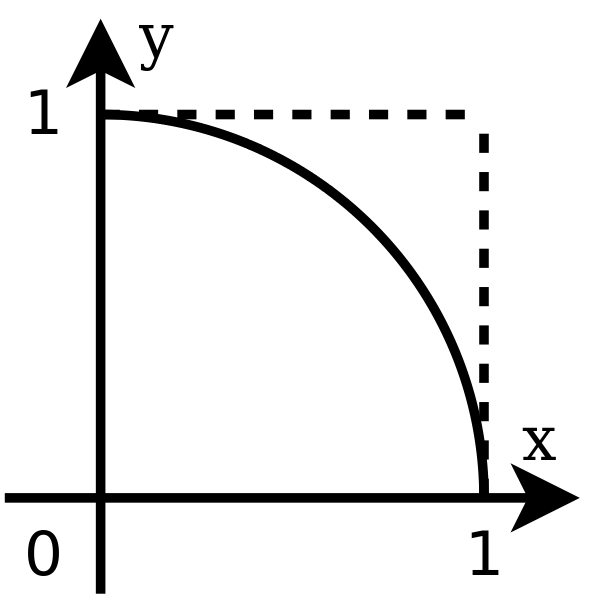
\includegraphics[width=0.9\textwidth]{pi.png}
\end{figure}
\end{column}
\end{columns}
\end{frame}

\begin{frame}
\frametitle{Square Root Algorithm}
TODO: Present a solution to the sqrt() task.
Concentrate of how the variable changes when iterating
\end{frame}

\begin{frame}
\frametitle{Case Study: Calulating $\pi$}
\begin{columns}
\begin{column}{0.6\textwidth}
\begin{itemize}
\small{
\item We can't calculate the area ratio without knowing $\pi$
\item Estimate it by:
\begin{itemize}
	\item Randomly picking many points inside the square
	\item Test if the point is inside the circle with $x^2 + y^2 < 1$
	\end{itemize}
}
\end{itemize}
\end{column}
\begin{column}{0.4\textwidth}
\begin{figure}
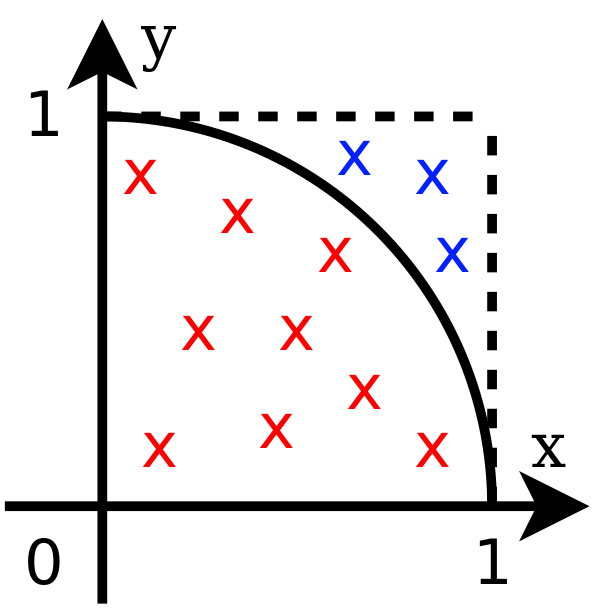
\includegraphics[width=0.9\textwidth]{pi-dots.png}
\end{figure}
\end{column}
\end{columns}
\begin{itemize}
\item $\pi \approx 4 \times \frac{\textrm{Number of points which land inside circle}}{\textrm{Total number of points tested}} = 4 \times \frac{9}{12} = 3$
\end{itemize}
\end{frame}

\begin{frame}[fragile]
\frametitle{Algorithm for Calculating $\pi$}
\begin{lstlisting}[style=pseudo]
BEGIN
	integer countTotal = 0
	integer countInside = 0
	WHILE countTotal < A large number
		x = random number between 0 and 1
		y = random number between 0 and 1
		countTotal = countTotal + 1
		IF x*x + y*y < 1
			countInside = countInside + 1
		ENDIF
	ENDWHILE
	pi = 4*countInside/countTotal
	PRINT pi
END
\end{lstlisting}
\end{frame}

\end{document}
